\documentclass{article}
\usepackage{graphicx}

\newcommand{\projectnaam}{Assignment: Working with Stride}
\newcommand{\student}{Johannes Akkermans}
\newcommand{\team}{
	\=Johannes Akkermans, \\\>Thomas Van Bogaert, \\\>Gilles De Borger, \\\>Siegfried Kriekemans, \\\>Zhong Xi Lu
}

\title{\textmd{\textbf{Bachelor eindwerk}}\\\normalsize\vspace{0.1in}\Large{\projectnaam}\\\vspace{0.1in}\small{\textit{3 Ba INF \  2017-2018}}}
\author{}

\begin{document}
\maketitle

\begin{center}
	\parbox{0cm}{
		\begin{tabbing}
		\textbf{Group:} \team
		\end{tabbing}
	}
\end{center}

\newpage
\section{Assignment}
\begin{center}
	\textit{Onderzoek het effect van verschillende R0 waarden op de attack rate.}
\end{center}

\section{Solution}
Om het verband te bepalen tussen de R0 en de attack rate is er 21 maal een simulatie uitgevoerd die telkens 50 dagen draait met verschillende waardes voor R0. De gekozen waardes voor R0 zijn 
$$\{0, 3, 6, 9, 12, 15, 18, 21, 24, 27, 30, 33, 36, 39, 42, 45, 48, 51, 54, 57, 60 \} $$

Met behulp van de \texttt{pystride} worden de 21 verschillende forks gesimuleerd en de resultaten zijn vervolgens te vinden in de \texttt{simulations} folder in de verschillende \texttt{summary.csv} bestanden. 

Hieronder zal er een overzicht gegeven worden van de verschillende attack rates bij de desbetreffende R0-waarde.

\begin{table}[h]
	\centering
	\begin{tabular}{ | l | r | }
		\hline			
		\textbf{R0} & \textbf{Attack Rate}  \\ \hline
0 & 0.002 \\
3 & 0.003015 \\
6 & 0.00483833 \\
9 & 0.00896 \\
12 & 0.01539 \\
15 & 0.0274583 \\
18 & 0.04412 \\
21 & 0.0657283 \\
24 & 0.0905667 \\
27 & 0.115945 \\
30 & 0.138522 \\
33 & 0.15693 \\
36 & 0.169693 \\
39 & 0.179667 \\
42 & 0.185718 \\
45 & 0.190217 \\
48 & 0.193123 \\
51 & 0.19524 \\
54 & 0.196977 \\
57 & 0.19795 \\
60 & 0.198903 \\
		\hline  
	\end{tabular}
	\caption{Results of the simulation}
\end{table}

\newpage
 
Wanneer de bovenstaande waardes worden weergegeven in een grafiek vormt deze een sigmo\"{i}dale curve; er is een geleidelijk snellere stijging met afzwakking bij hoge waarden. De reden dat de attack rate afzwakt, is omdat bij hoge R0 waardes, heel de bevolking (dat besmet kan worden) uiteindelijk besmet geraakt op de laatste dag, waardoor de attack rate ongeveer hetzelfde blijft en naar 0.2 convergeert.

\begin{figure}[h]
	\centering
	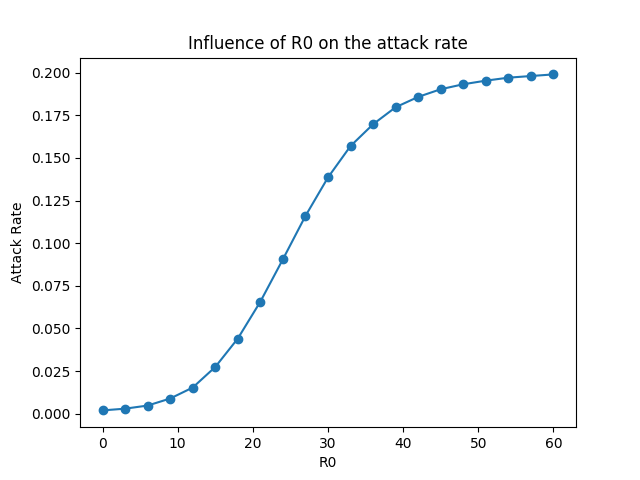
\includegraphics[width=\textwidth]{r0_2}
	\caption{Results of the simulation in a graph}
\end{figure}





\end{document}